\documentclass[draft]{scrartcl}

\usepackage[utf8]{inputenc}

\usepackage{fixltx2e}

\usepackage{microtype}
\usepackage{amsmath}
\usepackage{amssymb}
\usepackage{mathtools}
\usepackage{pgfplots}

% \usepackage{pgfplots}
% \pgfplotsset{compat=newest}
\DeclareMathOperator{\Conv}{Conv}

\newcommand\mytitle{Useful recurrence relations\\
for multidimensional volumes\\
and monomial integrals}
\newcommand\myauthor{Nico Schlömer}

\usepackage[
  pdfencoding=unicode,
  ]{hyperref}
\hypersetup{
  pdfauthor={\myauthor},
  pdftitle={Useful recurrence relations for multidimensional volumes and monomial integrals}
}

% \usepackage[T1]{fontenc}
% \usepackage{newtxtext}
% \usepackage{newtxmath}

% Okay. Don't use biblatex/biber for now. There are breaking changes in every revision,
% and we'd have to stick to the exact version that arxiv.org has, otherwise it's error
% messages like
% ```
% Package biblatex Warning: File 'main.bbl' is wrong format version
% - expected 2.8.
% ```
% \usepackage[sorting=none]{biblatex}
% \bibliography{bib}

\usepackage{bm}
\newcommand\rgb{\bm{R}}

\title{\mytitle\footnote{The LaTeX sources of this article are on
\url{https://github.com/nschloe/useful-recurrence-relations}}}
\author{\myauthor}

\begin{document}

\maketitle
\begin{abstract}
  Many mathematical entities, especially when working in arbitrary dimensions, are
  expressed in terms of the Gamma function, e.g., volume and surface of the hypersphere.
  These expressions are often complicated and don't provide much insight. Also, many
  expressions are unsuitable for use in a computer program. This note lists more
  suitable representations with recurrence relations for many common expressions.
\end{abstract}

\subsection*{\textit{n}-dimensional unit cube}
\[
  C_n = \left\{(x_1,\dots,x_n): -1 \le x_i \le 1\right\}
\]

\begin{itemize}
  \item Volume.
    \begin{equation}
      |C_n| = 2^n = \begin{cases}
        1&\text{if $n=0$}\\
        |C_{n-1}| \times 2&\text{otherwise}
      \end{cases}
    \end{equation}
  \item Monomial integration.
  \begin{equation}
    \begin{split}
    I_{k_1,\dots,k_n}
    &= \int_{C_n} x_1^{k_1}\cdots x_n^{k_n}\\
      &= \prod_{i=1}^n \frac{1 + (-1)^{k_i}}{k_i+1}
    =\begin{cases}
      0&\text{if any $k_i$ is odd}\\
      |C_n|&\text{if all $k_i=0$}\\
      I_{k_1,\dots,k_{i_0}-2,\dots,k_n} \times \frac{k_{i_0}-1}{k_{i_0}+1}&\text{if $k_{i_0} > 0$}
    \end{cases}
  \end{split}
  \end{equation}
\end{itemize}

\subsection*{\textit{n}-dimensional unit simplex}
\[
  T_n = \left\{(x_1,\dots,x_n):x_i \geq 0, \sum_{i=1}^n x_i \leq 1\right\}
\]

\begin{itemize}
  \item Volume.
    \begin{equation}
      |T_n| = \frac{1}{n!} = \begin{cases}
        1&\text{if $n=0$}\\
        |T_{n-1}| \times \frac{1}{n}&\text{otherwise}
      \end{cases}
    \end{equation}
  \item Monomial integration.
  % https://math.stackexchange.com/q/207073/36678
  \begin{equation}
    \begin{split}
    I_{k_1,\dots,k_n}
    &= \int_{T_n} x_1^{k_1}\cdots x_n^{k_n}\\
    &= \frac{\prod_{i=1}^n\Gamma(k_i)}{\Gamma\left(\sum_{i=1}^n k_i\right)}
    =\begin{cases}
      |T_n|&\text{if all $k_i=0$}\\
      I_{k_1,\dots,k_{i_0}-1,\dots,k_n} \times \frac{k_{i_0}}{\sum_{i=1}^n (k_i+1)}&\text{if $k_{i_0} > 0$}
    \end{cases}
  \end{split}
  \end{equation}
\end{itemize}

\subsection*{\textit{n}-dimensional unit sphere}
\[
  U_n = \left\{(x_1,\dots,x_n): \sum_{i=1}^n x_i^2 = 1\right\}
\]

\begin{itemize}
  \item Volume.
\begin{equation*}\label{ndimsphere}
  |U_n|
  = \frac{n \sqrt{\pi}^n}{\Gamma(\frac{n}{2}+1)}
  % = \begin{rcases}\begin{dcases}
  % \frac{n}{(\frac{n}{2})!} \pi^{\frac{n}{2}}&\text{if $n-1$ even}\\
  %   \frac{n2^{n+1}(\frac{n+1}{2})!}{(n+1)!}\pi^{\frac{n-1}{2}}&\text{if $n-1$ odd}
  % \end{dcases}
  % \end{rcases}
  = \begin{cases}
    2&\text{if $n = 1$}\\
    2\pi&\text{if $n = 2$}\\
    |U_{n-2}| \times \frac{2\pi}{n - 2}&\text{otherwise}
  \end{cases}
\end{equation*}

  \item Monomial integral \cite{folland}.
\[
  \begin{split}
  I_{k_1,\dots,k_n}
  &= \int_{U_n} x_1^{k_1}\cdots x_n^{k_n}\\
  &= 2 \frac{\prod_{i=1}^n
    \Gamma\left(\frac{k_i+1}{2}\right)}{\Gamma\left(\sum_{i=1}^n\frac{k_i+1}{2}\right)}
  =\begin{cases}
    0&\text{if any $k_i$ is odd}\\
    |U_n|&\text{if all $k_i=0$}\\
    I_{k_1,\dots,k_{i_0}-2,\dots,k_n} \times \frac{k_{i_0} - 1}{\sum_{i=1}^n (k_i+1) - 2}&\text{if $k_{i_0} > 0$}
  \end{cases}
  \end{split}
\]
\end{itemize}


\subsection*{\textit{n}-dimensional unit ball}
\[
  S_n = \left\{(x_1,\dots,x_n): \sum_{i=1}^n x_i^2 \le 1\right\}
\]

\begin{itemize}
  \item Volume.

\begin{equation}\label{ndimball}
  |S_n|
  = \frac{\sqrt{\pi}^n}{\Gamma(\frac{n}{2}+1)}
  % = \begin{rcases}
  %   \begin{dcases}
  %     \frac{\pi^{\frac{n}{2}}}{(\frac{n}{2})!}&\text{if $n$ even}\\[1.2ex]
  %     \frac{(\frac{n+1}{2})!2^{n+1}\pi^{\frac{n-1}{2}}}{\left(n+1\right)!}&\text{if $n$ odd}
  % \end{dcases}
  % \end{rcases}
  = \begin{cases}
     1&\text{if $n = 0$}\\
     2&\text{if $n = 1$}\\
     |S_{n-2}| \times \frac{2\pi}{n}&\text{otherwise}
  \end{cases}
\end{equation}

\item Monomial integral \cite{folland}.
\begin{equation}
  \begin{split}
    I_{k_1,\dots,k_n}
    &= \int_{S_n} x_1^{k_1}\cdots x_n^{k_n}\\
    &= \frac{2^p}{p} |S_n|
    =\begin{cases}
      0&\text{if any $k_i$ is odd}\\
      |S_n|&\text{if all $k_i=0$}\\
      I_{k_1,\dots,k_{i_0}-2,\dots,k_n} \times \frac{(k_{i_0} - 1)}{p - 2}&\text{if $k_{i_0} > 0$}
    \end{cases}
  \end{split}
\end{equation}
with $p=\sum_{i=1}^n (k_i+1)$.
\end{itemize}

\begin{figure}
\centering
% This file was created by tikzplotlib v0.9.2.
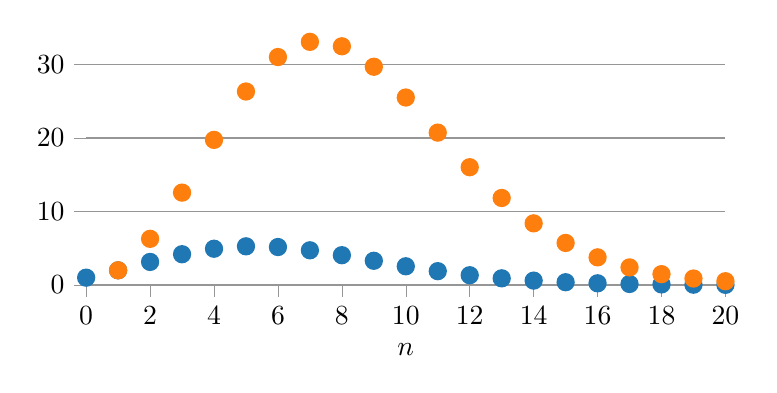
\begin{tikzpicture}

\definecolor{color0}{rgb}{0.12156862745098,0.466666666666667,0.705882352941177}
\definecolor{color1}{rgb}{1,0.498039215686275,0.0549019607843137}

\begin{axis}[
tick align=outside,
tick pos=left,
x grid style={white!58.8235294117647!black},
xlabel={$n$},
xmin=0, xmax=20,
xtick style={color=white!58.8235294117647!black},
y grid style={white!58.8235294117647!black},
ymajorgrids,
ymin=0.0258068913900141, ymax=33.0733617923198,
ytick style={color=white!58.8235294117647!black},
width={0.8\textwidth},
height={0.4\textwidth},
axis line style={draw=none},
ymin=0,
ymax=35
]
\addplot [semithick, color0, mark=*, mark size=3, mark options={solid}, only marks]
table {%
0 1
1 2
2 3.14159265358979
3 4.18879020478639
4 4.93480220054468
5 5.26378901391432
6 5.16771278004997
7 4.7247659703314
8 4.05871212641677
9 3.29850890273871
10 2.55016403987735
11 1.8841038793899
12 1.33526276885459
13 0.910628754783283
14 0.599264529320792
15 0.381443280823304
16 0.235330630358893
17 0.140981106917139
18 0.0821458866111282
19 0.0466216010300885
20 0.0258068913900141
};
\addplot [semithick, color1, mark=*, mark size=3, mark options={solid}, only marks]
table {%
1 2
2 6.28318530717959
3 12.5663706143592
4 19.7392088021787
5 26.3189450695716
6 31.0062766802998
7 33.0733617923198
8 32.4696970113341
9 29.6865801246484
10 25.5016403987734
11 20.7251426732889
12 16.0231532262551
13 11.8381738121827
14 8.38970341049109
15 5.72164921234956
16 3.76529008574229
17 2.39667881759136
18 1.47862595900031
19 0.885810419571682
20 0.516137827800281
};
\draw (axis cs:20.2,-0.641799437700104) node[
  scale=0.7,
  anchor= west,
  text=color0,
  rotate=0.0
]{n-ball};
\draw (axis cs:20.2,1.1837441568904) node[
  scale=0.7,
  anchor= west,
  text=color1,
  rotate=0.0
]{n-sphere};
\end{axis}

\end{tikzpicture}

  \caption{The volumes of the $n$-dimensional ball (and sphere) mysteriously peak at $5$
  (and $7$, respectively). The recurrence relations make it obvious why: The factor
  $\frac{2\pi}{n}$ ($\frac{2\pi}{n-2}$) becomes smaller than $1$.}
\end{figure}

\subsection*{\textit{n}-dimensional unit ball with Gegenbauer weight}
  % https://math.stackexchange.com/a/3695653/36678
  $\lambda > -1.$ (Compare with \eqref{ndimball} for $\lambda = 0$.)
\begin{itemize}
  \item Volume.
  \[
    \begin{split}
    |G_n^{\lambda}|
      &= \int_{S^n} \left(1 - \sum_{i=1}^n x_i^2\right)^\lambda\\
      &= \frac{
        \Gamma(1+\lambda)\sqrt{\pi}^n
      }{
        \Gamma\left(1+\lambda + \frac{n}{2}\right)
      }
      = \begin{cases}
        1&\text{for $n=0$}\\
        \frac{\Gamma(1+\lambda)\sqrt{\pi}}{\Gamma\left(\frac{3}{2} + \lambda\right)}&\text{for $n=1$}\\
        |G_{n-2}^{\lambda}|\times \frac{2\pi}{2\lambda + n}&\text{otherwise}
      \end{cases}
    \end{split}
  \]

  \item Monomial integration.
  \[
    \begin{split}
    I_{k_1,\dots,k_n}
      &= \int_{S^n} x_1^{k_1}\cdots x_n^{k_n} \left(1 - \sum_{i=1}^n
      x_i^2\right)^\lambda\\
      &= \frac{
        \Gamma(1+\lambda)\prod_{i=1}^n \Gamma\left(\frac{k_i+1}{2}\right)
      }{
        \Gamma\left(1+\lambda + \sum_{i=1}^n \frac{k_i+1}{2}\right)
      }\\
      &= \begin{cases}
        0&\text{if any $k_i$ is odd}\\
        |G_n^{\lambda}|&\text{if all $k_i=0$}\\
        I_{k_1,\dots,k_{i_0}-2,\dots,k_n} \times \frac{k_{i_0}-1}{2\lambda + \sum_{i=1}^n(k_i+1)}&\text{if $k_{i_0} > 0$}
      \end{cases}
    \end{split}
  \]
\end{itemize}


\subsection*{\textit{n}-dimensional unit ball with Chebyshev-1 weight}
% See [Wikipedia](https://en.wikipedia.org/wiki/Chebyshev_polynomials).

Gegenbauer with $\lambda=-\frac{1}{2}.$

\begin{itemize}
  \item Volume.
  \[
    \begin{split}
    |G_n^{-1/2}|
      &= \int_{S^n} \frac{1}{\sqrt{1 - \sum_{i=1}^n x_i^2}}\\
      &= \frac{
        \sqrt{\pi}^{n+1}
      }{
        \Gamma\left(\frac{n+1}{2}\right)
      }
      =\begin{cases}
        1&\text{if $n=0$}\\
        \pi&\text{if $n=1$}\\
        |G_{n-2}^{-1/2}| \times \frac{2\pi}{n-1}&\text{otherwise}
      \end{cases}
    \end{split}
  \]

  \item Monomial integration.
  \[
    \begin{split}
    I_{k_1,\dots,k_n}
      &= \int_{S^n} \frac{x_1^{k_1}\cdots x_n^{k_n}}{\sqrt{1 - \sum_{i=1}^n x_i^2}}\\
      &= \frac{
        \sqrt{\pi} \prod_{i=1}^n \Gamma\left(\frac{k_i+1}{2}\right)
      }{
        \Gamma\left(\frac{1}{2} + \sum_{i=1}^n \frac{k_i+1}{2}\right)
      }\\
      &= \begin{cases}
        0&\text{if any $k_i$ is odd}\\
        |G_n^{-1/2}|&\text{if all $k_i=0$}\\
        I_{k_1,\dots,k_{i_0}-2,\dots,k_n} \times \frac{k_{i_0}-1}{-1 + \sum_{i=1}^n(k_i+1)}&\text{if $k_{i_0} > 0$}
      \end{cases}
    \end{split}
  \]
\end{itemize}


\subsection*{\textit{n}-dimensional unit ball with Chebyshev-2 weight}
% See [Wikipedia](https://en.wikipedia.org/wiki/Chebyshev_polynomials).
Gegenbauer with $\lambda = +\frac{1}{2}.$

\begin{itemize}
  \item Volume.
  \[
    \begin{split}
    |G_n^{+1/2}|
      &= \int_{S^n} \sqrt{1 - \sum_{i=1}^n x_i^2}\\
      &= \frac{
        \sqrt{\pi}^{n+1}
      }{
        2\Gamma\left(\frac{n+3}{2}\right)
      }
      = \begin{cases}
        1&\text{if $n=0$}\\
        \frac{\pi}{2}&\text{if $n=1$}\\
        |G_{n-2}^{+1/2}| \times \frac{2\pi}{n+1}&\text{otherwise}
      \end{cases}
  \end{split}
  \]

  \item Monomial integration.
  \[
    \begin{split}
    I_{k_1,\dots,k_n}
      &= \int_{S^n} x_1^{k_1}\cdots x_n^{k_n} \sqrt{1 - \sum_{i=1}^n
      x_i^2}\\
      &= \frac{
        \sqrt{\pi}\prod_{i=1}^n \Gamma\left(\frac{k_i+1}{2}\right)
      }{
        2\Gamma\left(\frac{3}{2} + \sum_{i=1}^n \frac{k_i+1}{2}\right)
      }\\
      &= \begin{cases}
        0&\text{if any $k_i$ is odd}\\
        |G_n^{+1/2}|&\text{if all $k_i=0$}\\
        I_{k_1,\dots,k_{i_0}-2,\dots,k_n} \times \frac{k_{i_0}-1}{1 + \sum_{i=1}^n(k_i+1)}&\text{if $k_{i_0} > 0$}
      \end{cases}
    \end{split}
  \]
\end{itemize}


\subsection*{\textit{n}-dimensional generalized Laguerre volume}

$\alpha > -1.$

\begin{itemize}
  \item Volume.
\begin{equation*}\label{ndimlaguerre}
  \begin{split}
  V_n
    &= \int_{\mathbb{R}^n} \left(\sqrt{x_1^2+\dots+x_n^2}\right)^\alpha \exp\left(-\sqrt{x_1^2+\dots+x_n^2}\right)\\
    &= \frac{2 \sqrt{\pi}^n \Gamma(n+\alpha)}{\Gamma(\frac{n}{2})}
  % = \begin{rcases}\begin{dcases}
  %   \frac{2 \pi^{\frac{n}{2}} (n - 1)!}{(\frac{n}{2} - 1)!} &\text{if $n$ even}\\
  %   \pi^{\frac{n - 1}{2}} 2^n \left(\frac{n - 1}{2}\right)! &\text{if $n$ odd}
  % \end{dcases}
  % \end{rcases}
  = \begin{cases}
    2\Gamma(1+\alpha)&\text{if $n=1$}\\
    2\pi\Gamma(2 + \alpha)&\text{if $n=2$}\\
    V_{n-2} \times \frac{2\pi(n+\alpha-1) (n+\alpha-2)}{n-2}&\text{otherwise}
  \end{cases}
  \end{split}
\end{equation*}

\item Monomial integration.
\[
  \begin{split}
  I_{k_1,\dots,k_n}
  &= \int_{\mathbb{R}^n} x_1^{k_1}\cdots x_n^{k_n}
    \left(\sqrt{x_1^2+\dots+x_n^2}\right)^\alpha \exp\left(-\sqrt{x_1^2+\dots+x_n^2}\right)\\
  &= \frac{
    2 \Gamma\left(\alpha + \sum_{i=1}^n (k_i+1)\right)
    \left(\prod_{i=1}^n\Gamma\left(\frac{k_i + 1}{2}\right)\right)
  }{
    \Gamma\left(\sum_{i=1}^n\frac{k_i + 1}{2}\right)
  }\\
  &=\begin{cases}
    0&\text{if any $k_i$ is odd}\\
    V_n&\text{if all $k_i=0$}\\
    I_{k_1,\dots,k_{i_0}-2,\dots,k_n} \times \frac{
      (\alpha + p - 1) (\alpha + p - 2) (k_{i_0} - 1)
    }{
        p - 2
    }&\text{if $k_{i_0} > 0$}
  \end{cases}
  \end{split}
\]
with $p=\sum_{k=1}^n (k_i + 1)$.
\end{itemize}

\subsection*{\textit{n}-dimensional Hermite (physicists')}
\begin{itemize}
  \item Volume.
\[
  \begin{split}
  V_n
  &= \int_{\mathbb{R}^n} \exp\left(-(x_1^2+\dots+x_n^2)\right)\\
  &= \sqrt{\pi}^n
%   = \begin{rcases}\begin{dcases}
%      \pi^{\frac{n}{2}}&\text{if $n$ even}\\
%      \sqrt{\pi} \pi^{\frac{n-1}{2}}&\text{if $n$ odd}
%    \end{dcases}
%    \end{rcases}
   = \begin{cases}
     1&\text{if $n=0$}\\
     \sqrt{\pi}&\text{if $n=1$}\\
     V_{n-2} \times \pi&\text{otherwise}
   \end{cases}
  \end{split}
\]
%   \item Monomial 1D.
% % See [Wikipedia](https://en.wikipedia.org/wiki/Hermite_polynomials).
% \begin{equation*}
%   \begin{split}
%     I_k
%     &= \int_{-\infty}^\infty x^k \exp(-x^2) dx\\
%     &= \frac{(-1)^k + 1}{2} \times \Gamma\left(\frac{k+1}{2}\right)
%     % = \begin{cases}
%     % \frac{\sqrt{\pi}k!}{2^k (\frac{k}{2})!}&\text{if $k$ even}\\
%     % 0&\text{if $k$ odd}
%     % \end{cases}
%     = \begin{cases}
%       \sqrt{\pi}&\text{if $k = 0$}\\
%       0&\text{if $k = 1$}\\
%       I_{k-2} \times \frac{k-1}{2}&\text{otherwise}
%     \end{cases}
%   \end{split}
% \end{equation*}

  \item Monomial integration.
  \[
    \begin{split}
    I_{k_1,\dots,k_n}
    &= \int_{\mathbb{R}^n} x_1^{k_1}\cdots x_n^{k_n} \exp(-(x_1^2+\dots+x_n^2))\\
    &= \prod_{i=1}^n \frac{(-1)^{k_i} + 1}{2} \times \Gamma\left(\frac{k_i+1}{2}\right)\\
    &=\begin{cases}
      0&\text{if any $k_i$ is odd}\\
      V_n&\text{if all $k_i=0$}\\
      I_{k_1,\dots,k_{i_0}-2,\dots,k_n} \times \frac{k_{i_0} - 1}{2}&\text{if $k_{i_0} > 0$}
    \end{cases}
    \end{split}
  \]
\end{itemize}


\subsection*{\textit{n}-dimensional Hermite (probablisists')}
\begin{itemize}
  \item Volume.
\[
  V_n = \frac{1}{\sqrt{2\pi}^n} \int_{\mathbb{R}^n}
  \exp\left(-\frac{1}{2}(x_1^2+\dots+x_n^2)\right) = 1
\]

%   \item Monomial 1D.
% % https://en.wikipedia.org/wiki/Hermite_polynomials
% \[
%   \begin{split}
% I_k
%     &= \frac{1}{\sqrt{2\pi}} \int_{-\infty}^\infty x^k \exp\left(-\frac{1}{2}x^2\right) dx\\
%     &= \frac{(-1)^k + 1}{2} \times \frac{2^{\frac{k+1}{2}}}{\sqrt{2\pi}} \Gamma\left(\frac{k+1}{2}\right)
%     % = \begin{cases}
%     % \frac{k!}{2^{k/2} (\frac{k}{2})!}&\text{if $k$ even}\\
%     % 0&\text{if $k$ odd}
%     % \end{cases}
%     = \begin{cases}
%       1&\text{if $k = 0$}\\
%       0&\text{if $k = 1$}\\
%       I_{k-2} \times (k-1)&\text{otherwise}
%     \end{cases}
%   \end{split}
% \]

  \item Monomial integration.
  \[
    \begin{split}
    I_{k_1,\dots,k_n}
      &= \frac{1}{\sqrt{2\pi}^n} \int_{\mathbb{R}^n} x_1^{k_1}\cdots x_n^{k_n}
      \exp\left(-\frac{1}{2}(x_1^2+\dots+x_n^2)\right)\\
    &= \prod_{i=1}^n \frac{(-1)^{k_i} + 1}{2} \times
      \frac{2^{\frac{k_i+1}{2}}}{\sqrt{2\pi}} \Gamma\left(\frac{k_i+1}{2}\right)\\
    &=\begin{cases}
      0&\text{if any $k_i$ is odd}\\
      V_n&\text{if all $k_i=0$}\\
      I_{k_1,\dots,k_{i_0}-2,\dots,k_n} \times (k_{i_0} - 1)&\text{if $k_{i_0} > 0$}
    \end{cases}
    \end{split}
  \]
\end{itemize}


% \printbibliography{}
\bibliography{bib}{}
\bibliographystyle{plain}

\end{document}
